\chapter{Fundamentals of Machine Learning and Neural Networks}
\label{ml-fundamentals}

The promise of AI lies in the ability 
to integrate large amounts of data from huge data sets
and almost instantaneously register patterns
with clinical importance.

Machine Learning seeks to let computers learn from data
without them being explicitly programmed.


The Turing test, proposed by Alan Turing in 1950,
tries to answer the question \enquote{can a machine think?}.
A computer passes the test if a human interogator,
after posing a series of written questions,
cannot determine if the responses come from a human or a computer.


\textquote[russellArtificial2009]{%
The quest for \enquote{artificial flight} succeeded 
when engineers and inventors stopped imitating birds 
and started using wind tunnels and learning about aerodynamics.
Aeronautical engineering texts 
do not define the goal of their field as making 
\enquote{machines that fly so exactly like pigeons 
that they can fool other pigeons.}\,}

If the output is a finite set of values
the learning problem is called \textbf{classification},
and if it is a number, then it is called \textbf{regresion}.

In supervised learning, the model observes input-output pairs
and tries to learn a function that maps inputs to outputs.

In unsupervised learning, the model learns patterns in unlabeled input data.

With many machine-learning models, there is a bias--variance tradeoff:
on one end of the spectrum we have simple low-variance models 
such as linear or logistic regression
and on the other end, we have high-variance models
such as neural networks or random forests.

We can estimate the error rate of model
by evaluating it on a test set.
If we are only creating a single model,
then this approach suffices. 
However, we might want to compare many different models,
or slightly tweak an already existing model,
such that we can select the performing version.
If we select the final model based on the test set,
we might inadvertently have biased the process,
and could, in a sense, have overfitted to the test data.
To avoid this, we need to completely hide away the test data
until we are done with training, experimenting, 
and hyperparameter optimization.
To allow this, we instead need three sets of data:

\begin{itemize}
    \item a training set to train or develop candidate models
    \item a validation set to evaluate the candidate models
        and select the best one
    \item a test set do the final unbiased evaluation of model performance
\end{itemize}

Another alternative is using the technique \textit{k}-fold cross-validation.

A model is interpretable if we can inspect the model
and understand why it gave a certain output for a particular input.
An explainable model is one that can help us understand 
why a certain output was produced for a specific input.
Interpretability comes from inspecting the actual model.
Explainability can come from an external process.

Typically there is a distinction between model-based explanations
and post hoc explanations\autocite{vanderveldenExplainable2022}.
The scope of an explanation is the difference between
explanations for a complete model and
explanations for a single output.
Global explanation covers feature importance estimates 
for the entire dataset.
Local explanations, on the other hand, seeks to explain
the impact of the specific example under scrutiny.
A SHAP-waterfall plot is an example of a local explanation.
A saliency map of a chest radiograph that shows
which pixels contributed to the label \enquote{liver cancer}
is another example.

Shapley values measures the marginal contribution
of each individual feature.

One limitation of XAI models is the accuracy and relevance of explanations.
Explainability algorithms such as SHAP are only approximations
of the complete model.
In other words, the fidelity is not perfect and therefore neither
is the explanation.
However, for black-box models such as neural networks,
it is the next best thing.

\section{Neural Networks}

\begin{marginfigure}%
	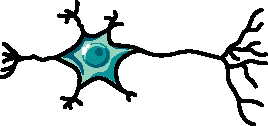
\includegraphics[width=\linewidth]{graphics/neuron}
    \caption[Schematic diagram of a neuron]{%
        Schematic diagram of a neuron.
        A typical neuron has a dendrites, a cell body, and a single axon; 
        the dendrites receive input signals from other neurons,
        and propagates output signals along the axon.
    }
    \label{fig:neuron}
\end{marginfigure}

\begin{marginfigure}%
	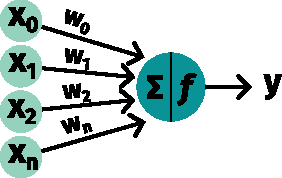
\includegraphics[width=\linewidth]{graphics/perceptron}
	\caption{Schematic diagram of a perceptron}
    \label{fig:perceptron}
\end{marginfigure}

%%%%%%%%%%%%%%%%%%%%%%%%%%%%%%%%%%%%%%%%%%%%%%%%%%%%%%%%%%%%%%%%%%%%%%%%%%%%%%%

Neural networks have been designed
using the archicteture of neurons in a human brain as inspiration.
The simplest model is that of a perceptron, 
which can be seen as a computational approximation
of a real neuron or nerve cell%
\autocite{charniakIntroduction2019}.
A typical neuron has many dendrites, a cell body, and a single axon 
(Figure~\ref{fig:neuron}).
The dendrites carries the input signal to a neuron,
and if the cumulative signal is great enough%
\sidenote{
    This threshold is known as 
    the \textit{threshold potential},
    and is typically between -50 and -55 mV.
}, 
then the neuron will propagate an action potential down the axon%
\autocite{seifterConcepts2005}.
In similar fashion, a perceptron receives may receive many different inputs
and produces a single output (Figure~\ref{fig:perceptron}).
In the case of a neuron, the \enquote{all-or-none} principle means
that nerve cells either signals at full strength or not all.
For a perceptron, this priniciple can be emulated
with the followingly step function:

\begin{equation}
    f_{\phi}(\mathbf{x})  = 
        \begin{cases}
            1 & \text{if } b + \mathbf{w} \cdot \mathbf{x} > 0\\
            0 & \text{otherwise}
        \end{cases}
\end{equation}

By combing many thousands of such neurons,
in a multilayer-perceptron or artificial neural network,
we can create a model that, 
can learn even the most complex of patterns.
Deep learning is at its core a form of representation learning.
Each layer in a neural network is a different representation,
and by stacking several of such layers on top of each others,
the representation in one hidden layer
feeds into the next layer and
is thereby being transformed into an even more abstract representation%
\autocite{estevaGuide2019}.

%%%%%%%%%%%%%%%%%%%%%%%%%%%%%%%%%%%%%%%%%%%%%%%%%%%%%%%%%%%%%%%%%%%%%%%%%%%%%%%
% insert example of abstract representations in a computervis model
%%%%%%%%%%%%%%%%%%%%%%%%%%%%%%%%%%%%%%%%%%%%%%%%%%%%%%%%%%%%%%%%%%%%%%%%%%%%%%%


\section{Regularization}

One approach to avoid overfitting in neural networks
is a technique known as dropout.
At each step of model training,
a random set of nodes in the network are disabled.
In a sense, the result is a rough approximation of 
an ensemble of different networks.


Dropout introduces noise during training
and thereby forces the network to be less senstive of noise.
Hidden units trained with dropout needs to be useful 
with or without the presence of neighboring units.

%%%%%%%%%%%%%%%%%%%%%%%%%%%%%%%%%%%%%%%%%%%%%%%%%%%%%%%%%%%%%%%%%%%%%%%%%%%%%%%

\section{Miscellaneous}

In his review on artificial intelligence in medicine%
\autocite{topolHighperformance2019}, 
Eric Topol expresses his view that in the future
\blockquote{%
almost every type of clinician, ranging from specialty doctor to paramedic,
will be using AI technology, and in particular deep learning [...]
}.

The ability to predict adverse outcomes could make  
healthcare resources more efficient.

Systematic deugging and continuous monitoring and validation 
is of utmost importance if we are to release AI algorithms into the wild%
\autocite{topolHighperformance2019}.

There has been much discussion about, and there are many opinions on, 
the black-box nature of many machine learning algorithms and 
how it should or should not affect the clinical use of such 
\autocite{topolHighperformance2019, gunningXAI2019, vanderveldenExplainable2022}.

In computer vision tasks in the medical domain,
deep-learning models have achieved physician-level performance
in many different diagnostic tasks
ranging from \todo{finish sentence}.

Automated diagnosis in ophthalmology 
from optical coherence tomography scans~\autocite{defauwClinically2018}.

\section{Computational models in cardiology}

Using single-lead lectrocardiogram recordings from \num{53877} patients,
Hannun et al.\autocite{hannunCardiologistlevel2019}
constructed a deep neural network
to identify 12 difference classes of cardiac rythm.
In the validation of their algorithm on an independent test set,
the authors were able to show that the computer model
significantly outperforms the average cardiologist. 

As the amount of available diagnostic data increases,
it becomes more difficult for the treating physician
to fully utilize the complete array of phenotypic information.
Computational models can easily integrate all this data,
and through automated identification of important clinical patterns
they could serve as an important diagnostic support.

\vskip 10em

Historically, artificial neural networks (ANNs) have been predominantly
employed for classification tasks, such as those typically found 
in image recognition and natural language processing. 
However, advancements have expanded their applicability, allowing ANNs 
to be tailored for handling time-to-event data.
This extension is particularly useful in fields like healthcare and systems
biology, where survival analysis or event prediction over a time horizon is
critical. 
While the present chapter will not delve further into machine learning
applications for time-to-event data, the topic will be revisited in the
subsequent chapter.

